\documentclass[main.tex]{subfiles}
\begin{document}

\section{Umsetzung}
In diesem Abschnitt werden die Details der Implementationen auf den beiden Smartphone-Plattformen iOS und Android, sowie den Aufbau unserer ARDoor Library beschrieben.

\subsection{Grundarchitektur}
Wir haben die Grundarchitektur unserer Applikation laut der Abbildung \ref{fig:android-architecture} definiert. Die einzelnen Komponenten werden hier kurz beschrieben.

\paragraph{OpenCV}
ist ein quasi-Standard in der nativen Bildverarbeitung und untersützt eine Vielzahl an Bearbeitungsfunktionen. OpenCV wird in der ARDoor Library für die Bildverarbeitung verwendet.

\paragraph{OpenGL}
wird für das 3D-Rendering benötigt. In der mobilen Welt ist die Library mittlerweile Standard und wird von Android und iOS unterstützt.

\paragraph{ARDoor C++ Library}
Die ARDoor Library enthält den Hauptteil der Applikation. In ihr wird sämtliche plattformunabhängige Logik sowie Verarbeitung und Rendering implementiert. C++ eignet sich  dafür gut, da sowohl von iOS via Objective-C als auch von Android über JNI auf die Library zugegriffen werden kann.

\paragraph{Plattformspezifischer Client}
Pro Plattform wird ein eigener Client implementiert, der den Kamerazugriff übernimmt. Die erfassten Einzelbilder werden an die ARDoor Library zur verarbeitung weitergereicht. Dieser Client sollte nur als Zwischenschicht dienen und deshalb so schlank wie möglich gehalten werden. 


\begin{figure}[!ht]
\centering
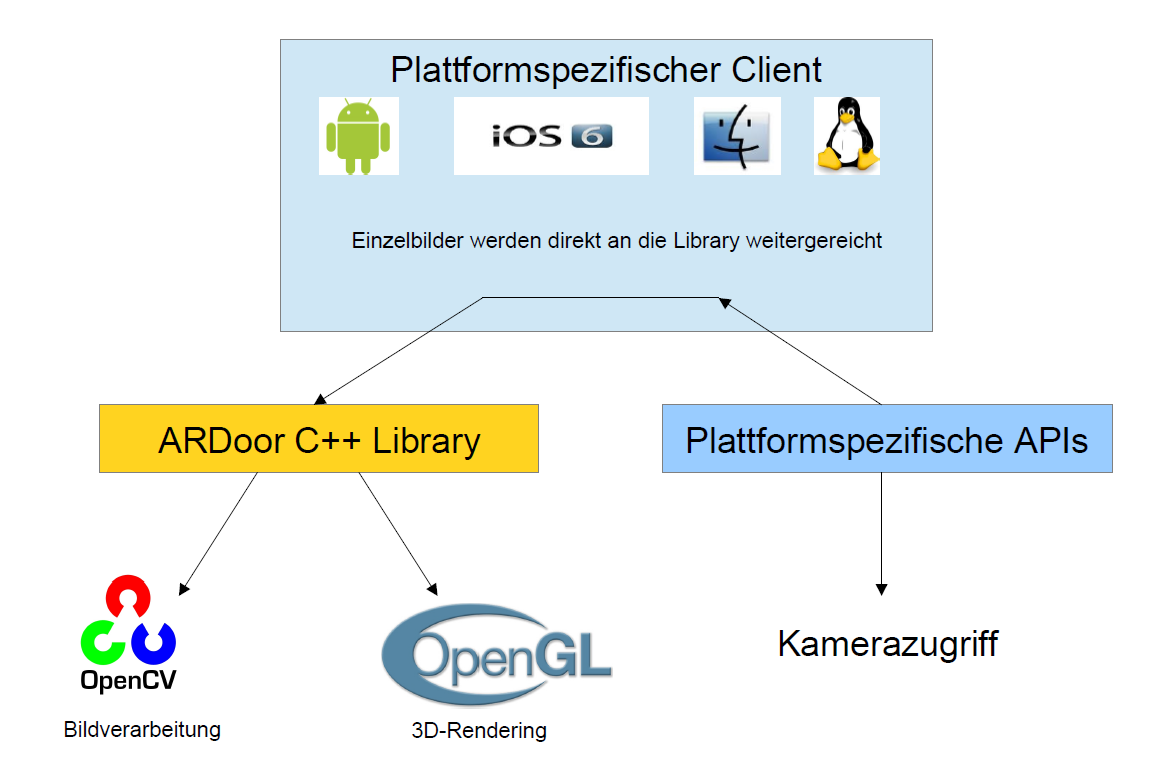
\includegraphics[scale=0.4]{images/architecture.png} 
\caption{Grundarchitektur von ARDoor}
\label{fig:android-architecture}
\end{figure}

\subsection{Android Plattform}
Zur Entwicklung und zum Testen unter Android wurde ein etwas in die Jahre gekommenes HTC Desire Z verwendet. Es wurde jedoch eine Custom Firmware aufgespielt, welche der Android Version 2.3 entspricht, um bessere Native-Unterstützung zu erhalten. Seit dieser Version, welche dem API Level 9 entspricht, gibt es u.a. die Möglichkeit, eine Native Activity zu implementieren.


\subsubsection{Native Activity}
Eine Native Activity ist seit Android 2.3 (API Level 9) verfügbar. Eine Native Activity ist im Grunde ein nützlicher Weg, um eine Android App in C/C++ zu implementieren, ohne noch zusätzlichen Wrapper-Code in Java und JNI Code zu schreiben. Mittels der dem Android NDK beiliegenden Library android\_native\_app\_glue kann das Grundgerüst der Native Activity in C/C++ implementiert werden. Dies hat jedoch einige Probleme bereitet.

\paragraph{}
Eines der Probleme war, dass primär zur Entwicklung unter Android Java (via Dalvik VM) als Programmiersprache vorgesehen ist. Ein Grossteil der verfügbaren APIs ist aus diesem Grund nur über Java aufrufbar. Dazu gehört auch die API für den Kamerazugriff. Es wäre zwar möglich aus C++ über JNI mit der Java-API zu kommunizieren, jedoch ist dies aufwändig und fehleranfällig. Auch verursacht JNI einen gewissen Overhead, wodurch ein Aufruf der rein in Java implementierten APIs aus Java-Code heraus schneller ist. JNI Code ist ausserdem sehr mühsam zum lesen und verursacht hohen Wartungsaufwand.

\paragraph{}
Es gibt auch die Möglichkeit mittels der OpenCV Capture-API auf die Kamera des Smartphones zuzugreifen. Das Problem dabei ist, dass OpenCV dazu undokumentierte Funktionen aus einer Android System-Library aufruft. Dies funktioniert leider nicht mit allen Geräten. Da die aufgerufenen Funktionen nicht zu einer offiziellen, stabilen API gehören, können diese bei einer neuen Android-Version ändern und die Entwickler von OpenCV müssten diese Unterstützung zuerst implementieren.

\paragraph{}
Was bei der Native Activity auch beachtet werden muss ist, dass die ganzen Android-Events, z.B. Input oder App-Lifecycle-Events, selber abgeholt und weiterverarbeitet werden müssen. Dadurch schreibt man quasi von Grund auf ein eigenes Applikationsframework auf nativer Basis.


\subsubsection{JNI Zugriff}
Die andere Möglichkeit ist der Zugriff auf C/C++ via JNI. Die Grund-App wird dabei in Java implementiert. In der nativen Library werden bei dieser Methode spezielle JNI-Funktionen implementiert, die aus Java heraus aufgerufen werden können.

\paragraph{}
Bei dieser Variante haben wir zwar immer noch die Java-Schicht, jedoch kann dadurch auf eine stabile und funktionierende API zurückgegriffen werden. Auch ist es einfacher später ein GUI zu implementieren, z.B. zur Auswahl des zu projizierenden 3D-Models.


\subsection{iOS Plattform}



\subsection{ARDoor Library}




\end{document}
